\section{Participants}
\label{sec:participants}
Ninety-one participants were recruited from Ontario Tech University's undergraduate student body through SONA. 
Participation flow is illustrated in Figure \ref{fig:participants_sankey}. 
Four participants were removed due to equipment recording issues. 
Participants were then screened on inclusion criteria for a) task attention, and b) fNIRS signal quality. 
For attention, participants were required to achieve $>=$ 60\% accuracy on the behavioral memory task (chance accuracy = 50\%) to ensure sufficient engagement. 
One participant failed to meet this criterion. 
The remaining 87 participants (69 females and 18 males, M = 21.09, SD = 5.91, range = 17 to 51) were analyzed in the behavioral memory task.
For neural analyses, signal quality of remaining 87 participants by computing the Peak Spectral Power (PSP) and the Scalp Coupling Index (SCI) \citep{pollonini_phoebe_2016}.
Measures were calculated using a 5-second sliding window across all channels \citep{bulgarelli_growth_2025, hernandez_nirsplot_2020}. 
fNIRS inclusion criteria were:
1) PSP $>$ 0.1 and SCI $>$ 0.5 for more than 70\% of the windows in a single channel, labelled "good signal quality" \citep{holmes_opening_2024}, and 
2) $>$ 70\% of the channels for a single participant were marked as "good". 
Thirty-five participants failed to meet these criteria, illustrated in Figure \ref{fig:signal_quality}, and were removed prior to data analysis. 
The final sample consisted of 52 participants (39 females and 13 males, M = 21.62, SD = 6.67, range = 17 to 51). 

\begin{figure}[H]
    \centering
    \begin{subfigure}[b]{0.75\textwidth}
        \centering
        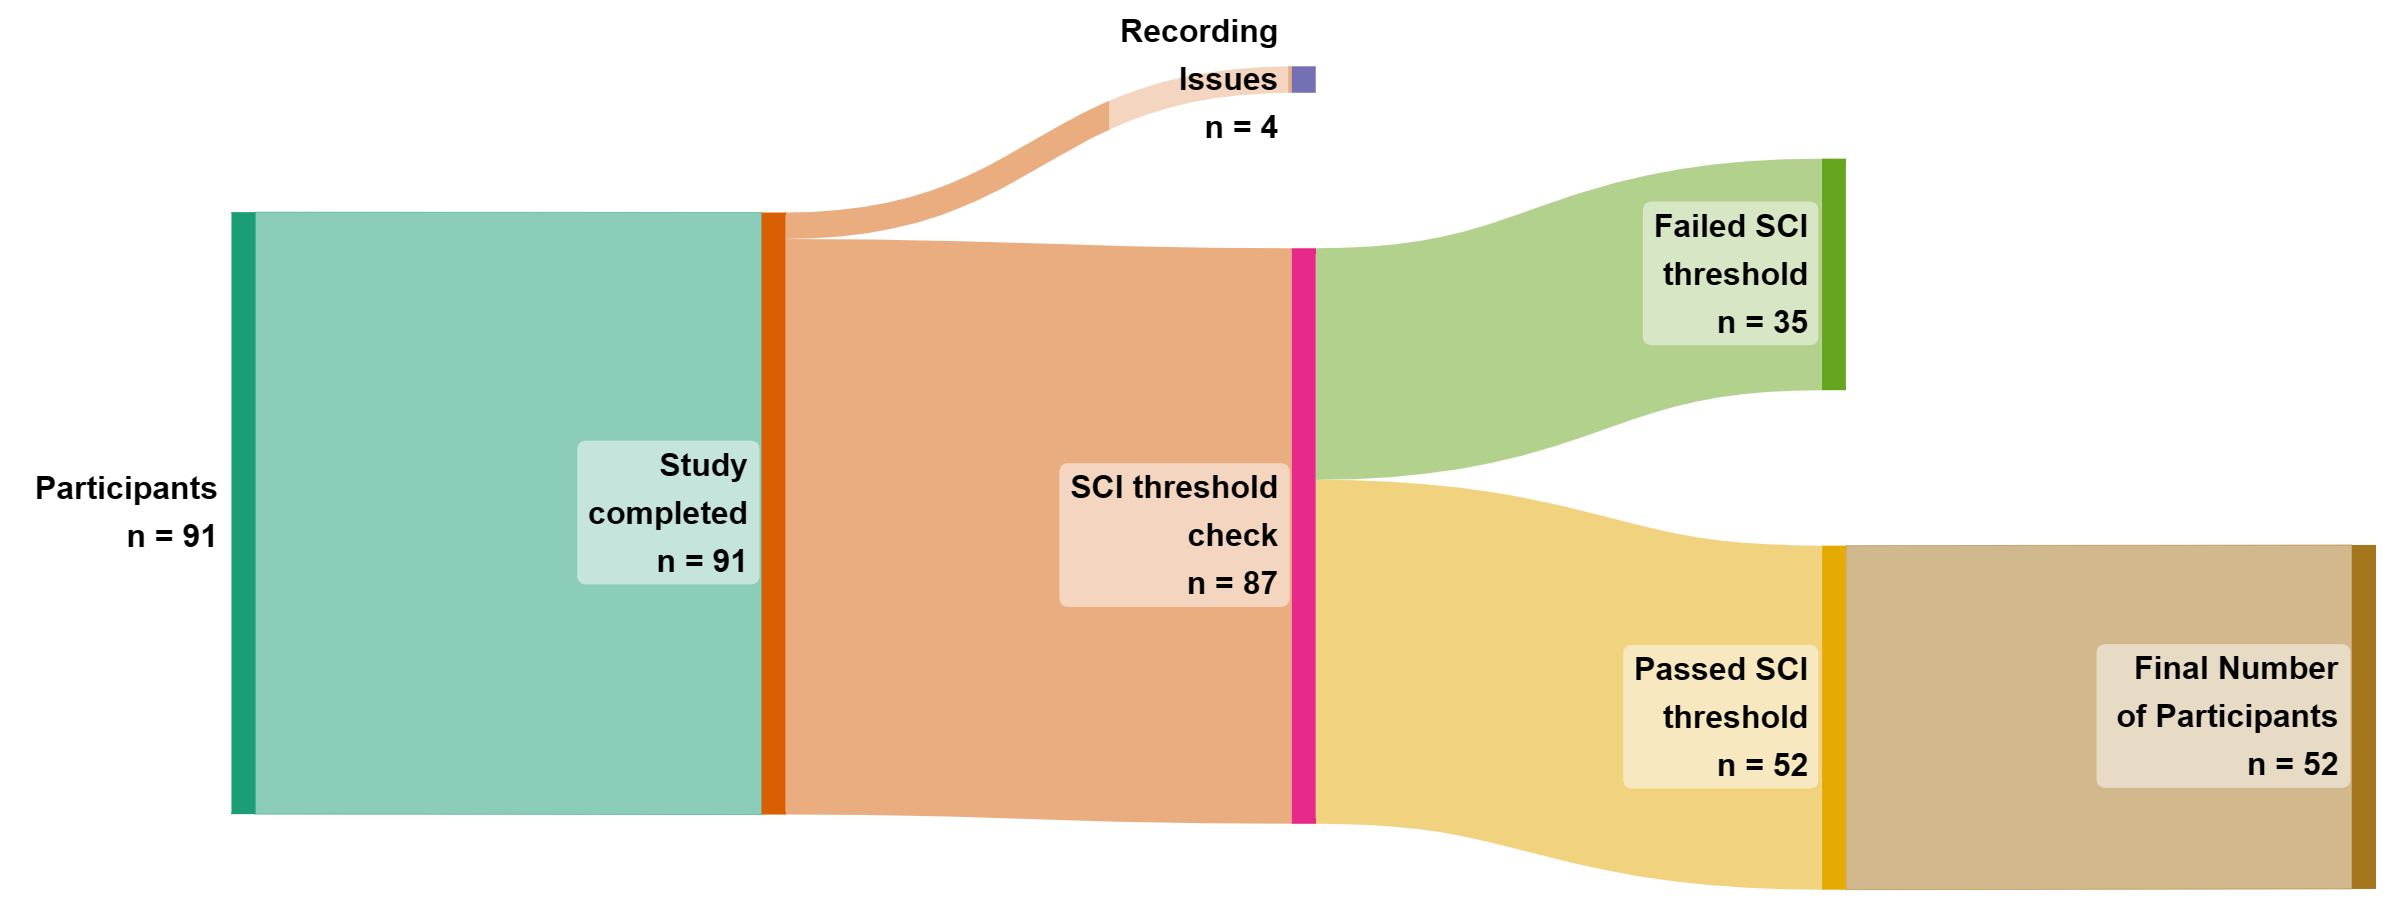
\includegraphics[width=\textwidth]{C:/Users/super/OneDrive - Ontario Tech University/fNIRS_Emotions/plots/figures/Participants Sankey Diagram.png}
        \caption[Participant inclusion flow diagram]{Sankey diagram showing the flow of participants through each stage of inclusion/exclusion in the study.}
        \label{fig:participants_sankey}
    \end{subfigure}
    \vskip\baselineskip
    \begin{subfigure}[b]{0.85\textwidth}
        \centering
        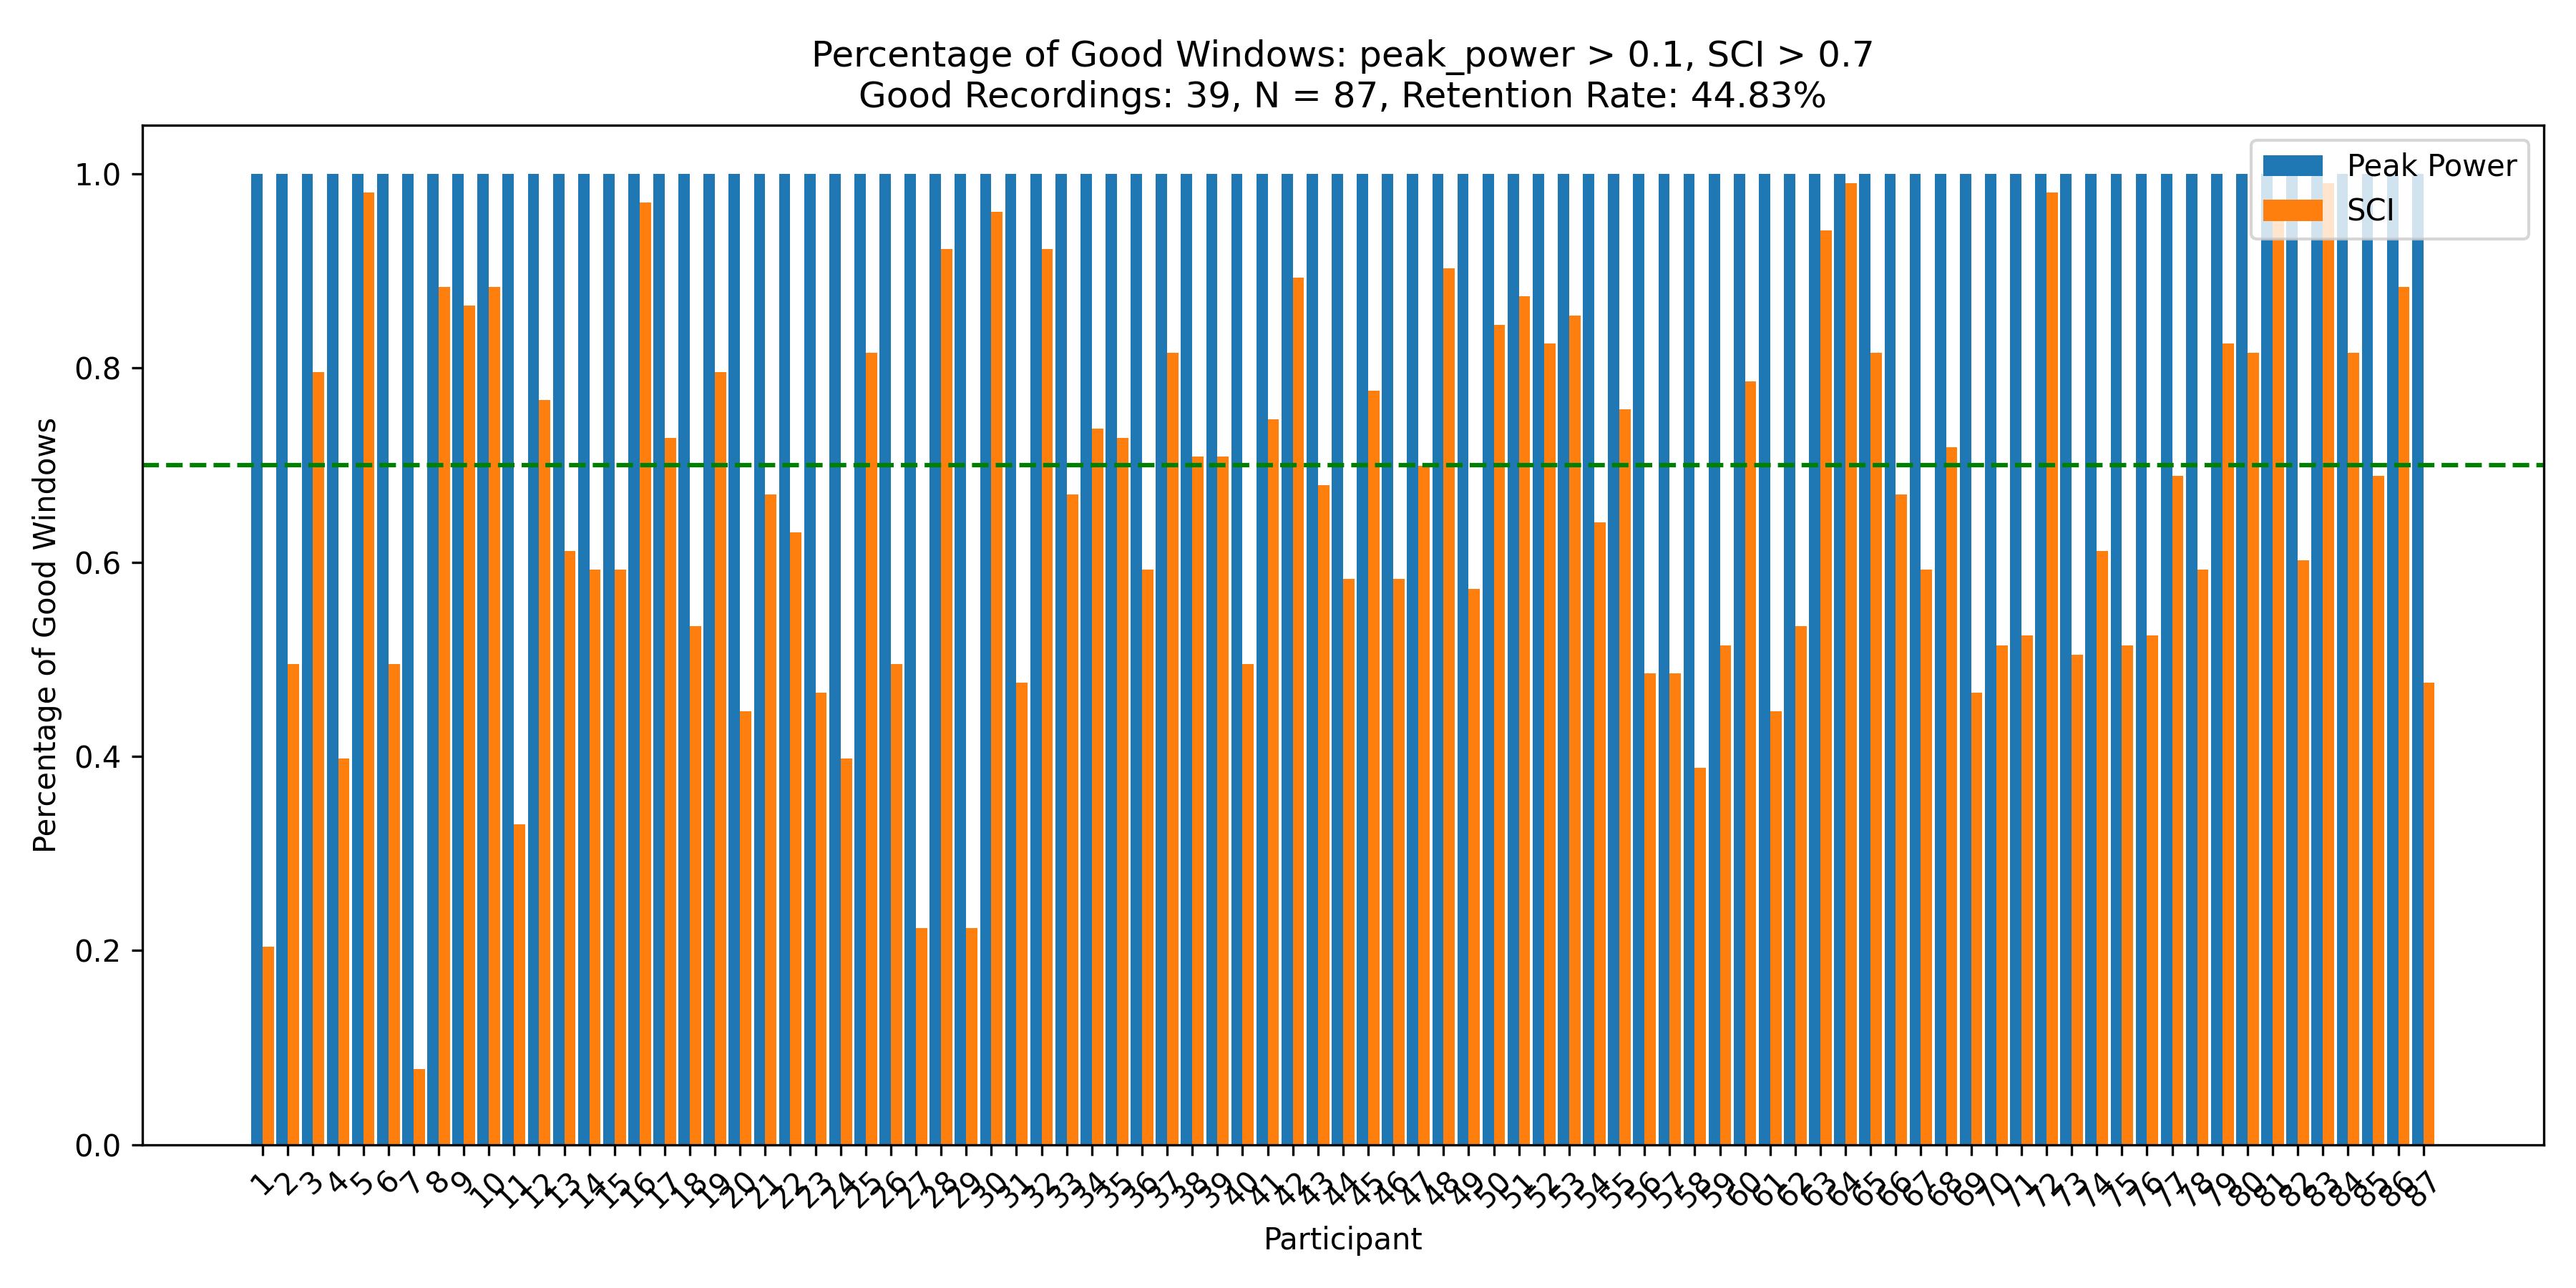
\includegraphics[width=\textwidth]{C:/Users/super/OneDrive - Ontario Tech University/fNIRS_Emotions/plots/signal quality/Percentage of Good Windows.png}
        \caption[SCI signal quality inclusion threshold]{Percentage of Channels where SCI $>$ 0.5 for $>$ 70\% of the windows.
        The green dashed line represents the threshold of 70\% of windows that each participant must meet to be included in the analysis.}
        \label{fig:signal_quality}
    \end{subfigure}
    \caption[Participant signal quality and inclusion flow]{(A) Participant inclusion flow diagram. (B) SCI signal quality inclusion threshold.}
    \label{fig:signal_quality_and_sankey}
\end{figure}

\section{Stimuli and apparatus}
\subsection{Stimuli}
One hundred and forty images of facial expressions from the racially diverse affective expression (RADIATE) and UIBVFED datasets were used \citep{conley_racially_2018, oliver_uibvfed_2020}.
The RADIATE contains perceptually validated images of racially and ethnically diverse participants, aged 18-30 years old, each expressing 16 different emotions. 
The UIBVFED dataset contains a set of 20 virtual characters that are also ethnically diverse, aged 20-80 years old expressing 32 emotions. 
The UIBVFED facial expressions were created using blendshapes, a tool that represents and manipulates clusters of facial landmarks similar to that of facial action units (AUs).
Then adult models (5 males and 5 females) from each dataset were identified and matched between-sets on face shape, sex, skin tone, and hair colour. 
Images of each model expressing seven emotions (anger, disgust, fear, happiness, sadness, surprise, neutral) were selected. 
Expressions were selected for each model, that closely align with Ekman's 6 basic emotions + neutral \citep{ekman1971constants}.
UIBVFED images were cropped to the same size as RADIATE images. 

\subsection{Apparatus}
Participants were tested individually in a quiet dedicated testing room. 
Stimuli were presented on a Dell U2415 24-inch monitor at 1920x1200 60Hz. 
Participants were seated in a comfortable non-movable chair, with the monitor placed at eye level. 
Stimuli were presented using PsychoPy3 Experiment Builder (v2024.1.5) \citep{peirce_psychopy2_2019}. 
Participant brain activity was recorded using Aurora fNIRS while participants completed the task. 
fNIRS data was collected using two NIRSport2 systems (NIRx Medical Technologies, Berlin, Germany). 
Each NIRSport2 system was equipped with 16 source and 16 detector optodes, and daisy-chained together for a high density 32x32 optode configuration. 
Each neighboring pair of source and detector optode is referred to as a channel, resulting in a total of 103 HbO + 103 HbR channels (plus 16 short distance channels).
The average distance between source and detector optodes was 30 mm, and 7mm for short distance channels, which were placed on a flexible fNIRS head cap (NIRScap) 58 cm in circumference. 
The optodes were arranged in a high density 32x32 montage with one bundle of short distance channels, as shown in Figure \ref{fig:montage_combined}.
This montage was designed to cover a maximally large area of the brain, given increasing evidence that emotion processing is not localized to specific discrete areas of the brain, rather distributed across the brain \citep{lindquist_brain_2012}. 
The fNIRS cap and optodes were positioned following the 10-20 international coordinate system.
Light was emitted at 760 nm and 850 nm wavelengths, and the sampling rate was approximately 6.105 Hz.

\begin{figure}[H]
    \centering
    \begin{subfigure}[b]{0.69\textwidth}
        \centering
        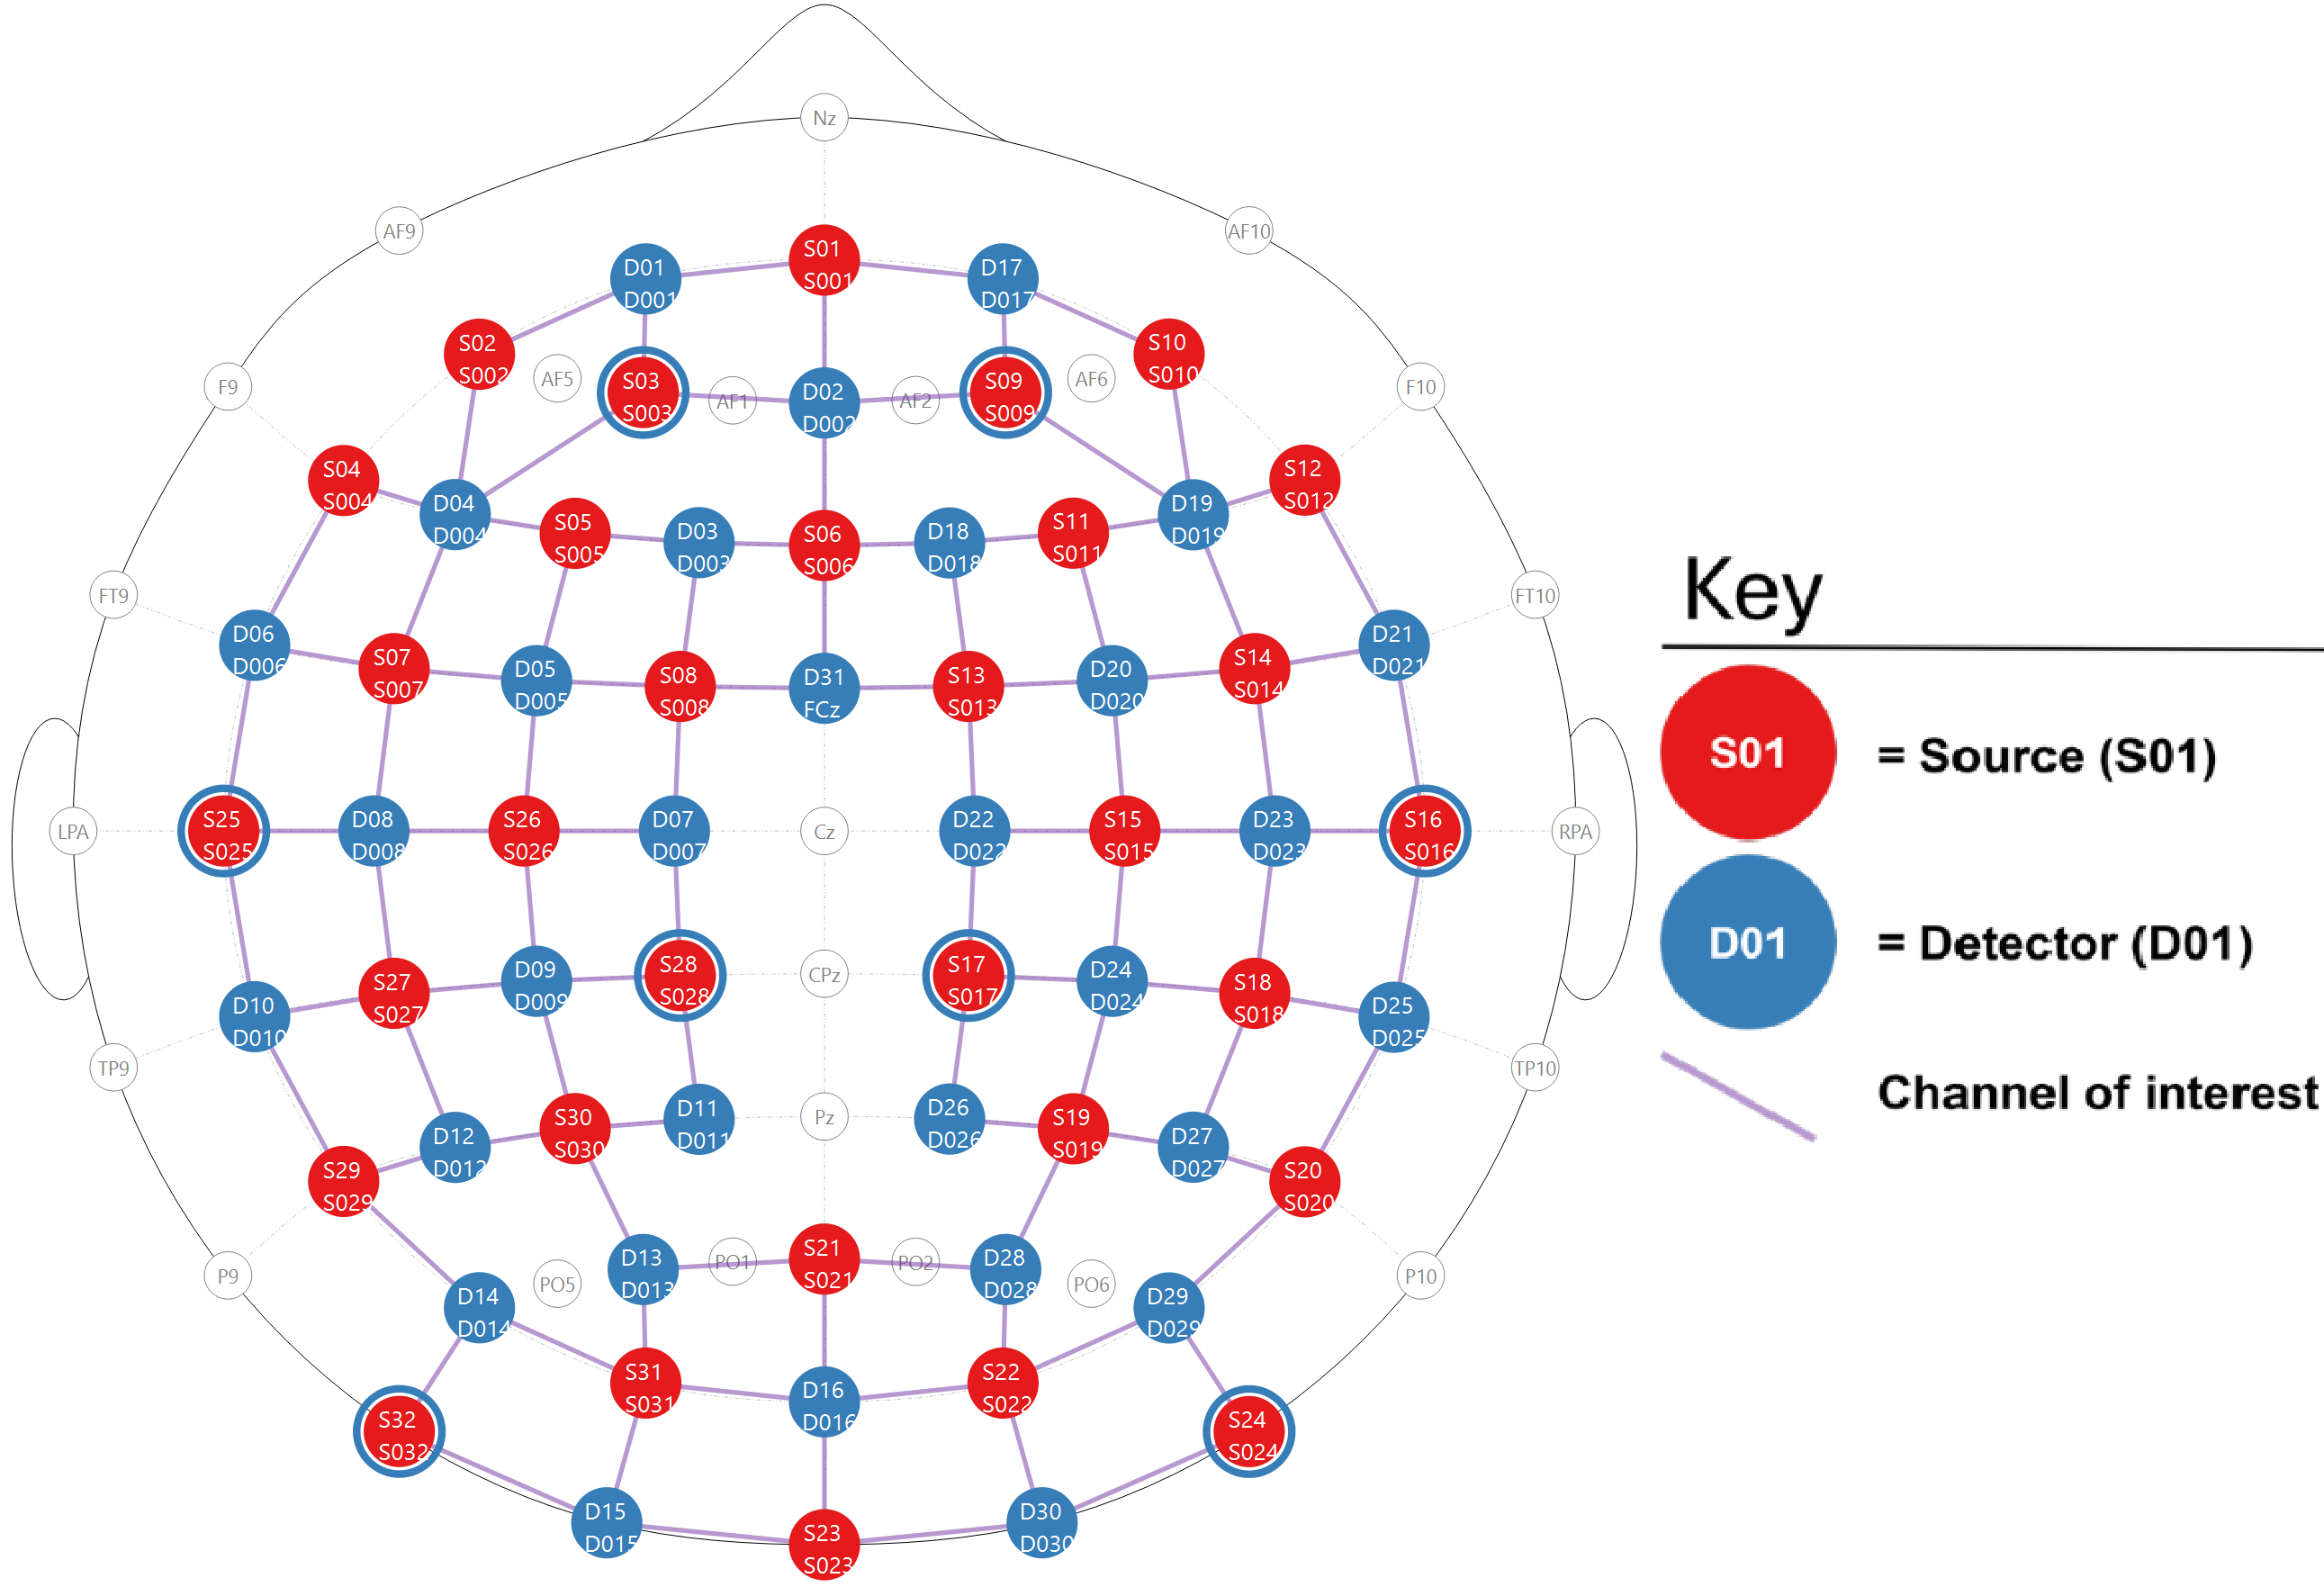
\includegraphics[width=\textwidth]{C:/Users/super/OneDrive - Ontario Tech University/fNIRS_Emotions/plots/figures/Montage.png}
        \caption[Montage depictions]{}
        \label{fig:montage}
    \end{subfigure}
    \hfill
    \begin{subfigure}[b]{0.3\textwidth}
        \centering
        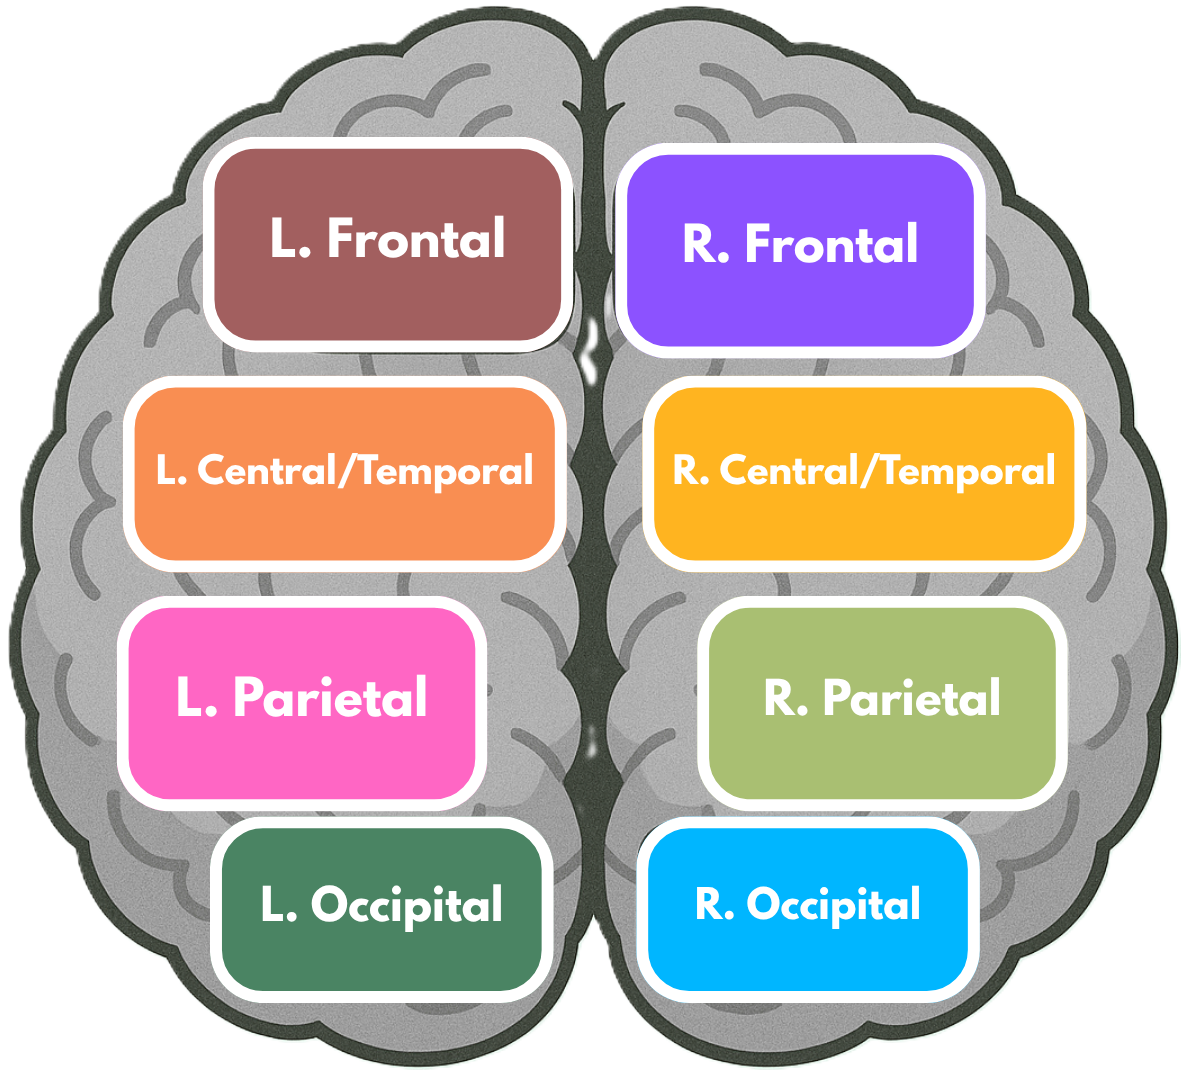
\includegraphics[width=\textwidth]{C:/Users/super/OneDrive - Ontario Tech University/fNIRS_Emotions/plots/figures/Brain Region Map.png}
        \caption[Brain region map for ROI grouping]{}
        \label{fig:brain_region_map}
    \end{subfigure}
    \caption[Montage and brain region map]{(a) Depictions of the high density 32x32 optode montage. Red circles represent sources, blue circles represent detectors, the colored lines represent channels, and blue rings around sources represent the locations of the 8 short distance detectors.
        The colors of the channels represent the regions of interest (ROI's) that the channels were grouped into. (b) Brain region map, showing the regions of interest (ROI's) that the channels were grouped into for certain analyses.}
    \label{fig:montage_combined}
\end{figure}

\section{Design and procedure}
\subsection{Design}
\label{sec:Design}
A full-factorial Face-type (2 levels: Real, Virtual) \texorpdfstring{$\times$}{x} Emotion (7 levels: Anger, Disgust, Fear, Joy, Sadness, Surprise, Neutral) \texorpdfstring{$\times$}{x} Model (4) \texorpdfstring{$\times$}{x} Sex (2 levels: Male, Female) \texorpdfstring{$\times$}{x} Repetition (4) experimental design was used, with each participant presented with 448 images. 
Stimuli were blocked and counterbalanced by Face-type and Emotion. 
Within each of the 56 Face-type-Emotion Blocks, participants were presented with 8 distinct model faces (4 male, 4 female).

\subsection{Planned analyses and preregistration}
This project was preregistered on the Open Science Framework before any data were collected (OSF DOI: \href{https://doi.org/10.17605/OSF.IO/76Q8W}{10.17605/OSF.IO/76Q8W}).
The preregistration document, time-stamped on 2 February 2024, specifies the study design, sampling plan, variables, and analysis plan.
By making the protocol public, we aimed to reduce analytic flexibility, enhance reproducibility, and enable independent verification of all planned and exploratory analyses.
Several elements of the preregistration were intentionally deferred or modified in the present thesis. 
First, although the OSF protocol outlines a linear mixed-effects model (LMM), those analyses were always earmarked for publication in a journal paper and are therefore not reported here. 
Second, the preregistered exploratory machine-learning (ML/AI) classifiers that were intended to decode Face-type and Emotion from multivariate HbT patterns, were not implemented due to time constraints and will be pursued in future work.  

\subsection{Procedure}
\label{sec:Procedure}
Following consent and briefing, participant head size was measured and a size-appropriate fNIRS cap fitted. 
A signal optimization routine was then run within Aurora fNIRS to optimize participant channel signal levels. 
This routine worked by increasing source brightness in a stepwise manner, until the optimal signal levels for all channels was reached. 
Following optimization, participants were told that they would be presented with a series of facial expression images and asked to identify whether a probe face matched one of the faces they saw in the preceding block. 
Room lights were then switched off to avoid interference with the fNIRS cap, and participants were monitored from an adjacent room with a live camera feed. 

The experiment began with instructions presented on screen. 
The trial timeline, shown in Figure \ref{fig:paradigm}, consisted of three main epochs: fixation cross, block presentation, and participant feedback. 
Each Block began with a fixed cross presented for 16 seconds, followed by 8 facial images. 
Facial images were each presented for 1.5 seconds, with a 250-750 ms (M=500 ms) interstimulus interval (ISI) between each face. 
To maintain participant attention, participants completed a memory task after each block. 
In the task, participants were presented with a model image with the same emotional expression as the rest of the block's images, and asked if the model was shown in the preceding block of 8 faces, with feedback provided using the keyboard (y/n). 
The probe face has a 50\% chance of either being in the previous block or not. 
The experiment continued after seven seconds if no feedback was provided (the distribution of block missed responses is shown in Appendix \ref{fig:appendix_memory_task_no_response_distribution}).
Participants were given a break every seven blocks, and prompted to enter the space bar when they are ready to continue the experiment. 
After the experiment was completed, the experimenter(s) entered the room, removed the fNIRS cap, and the participant was debriefed about the experiment. 
Participation in the experiment took approximately 35 minutes.

\begin{figure}[H]
    \centering
    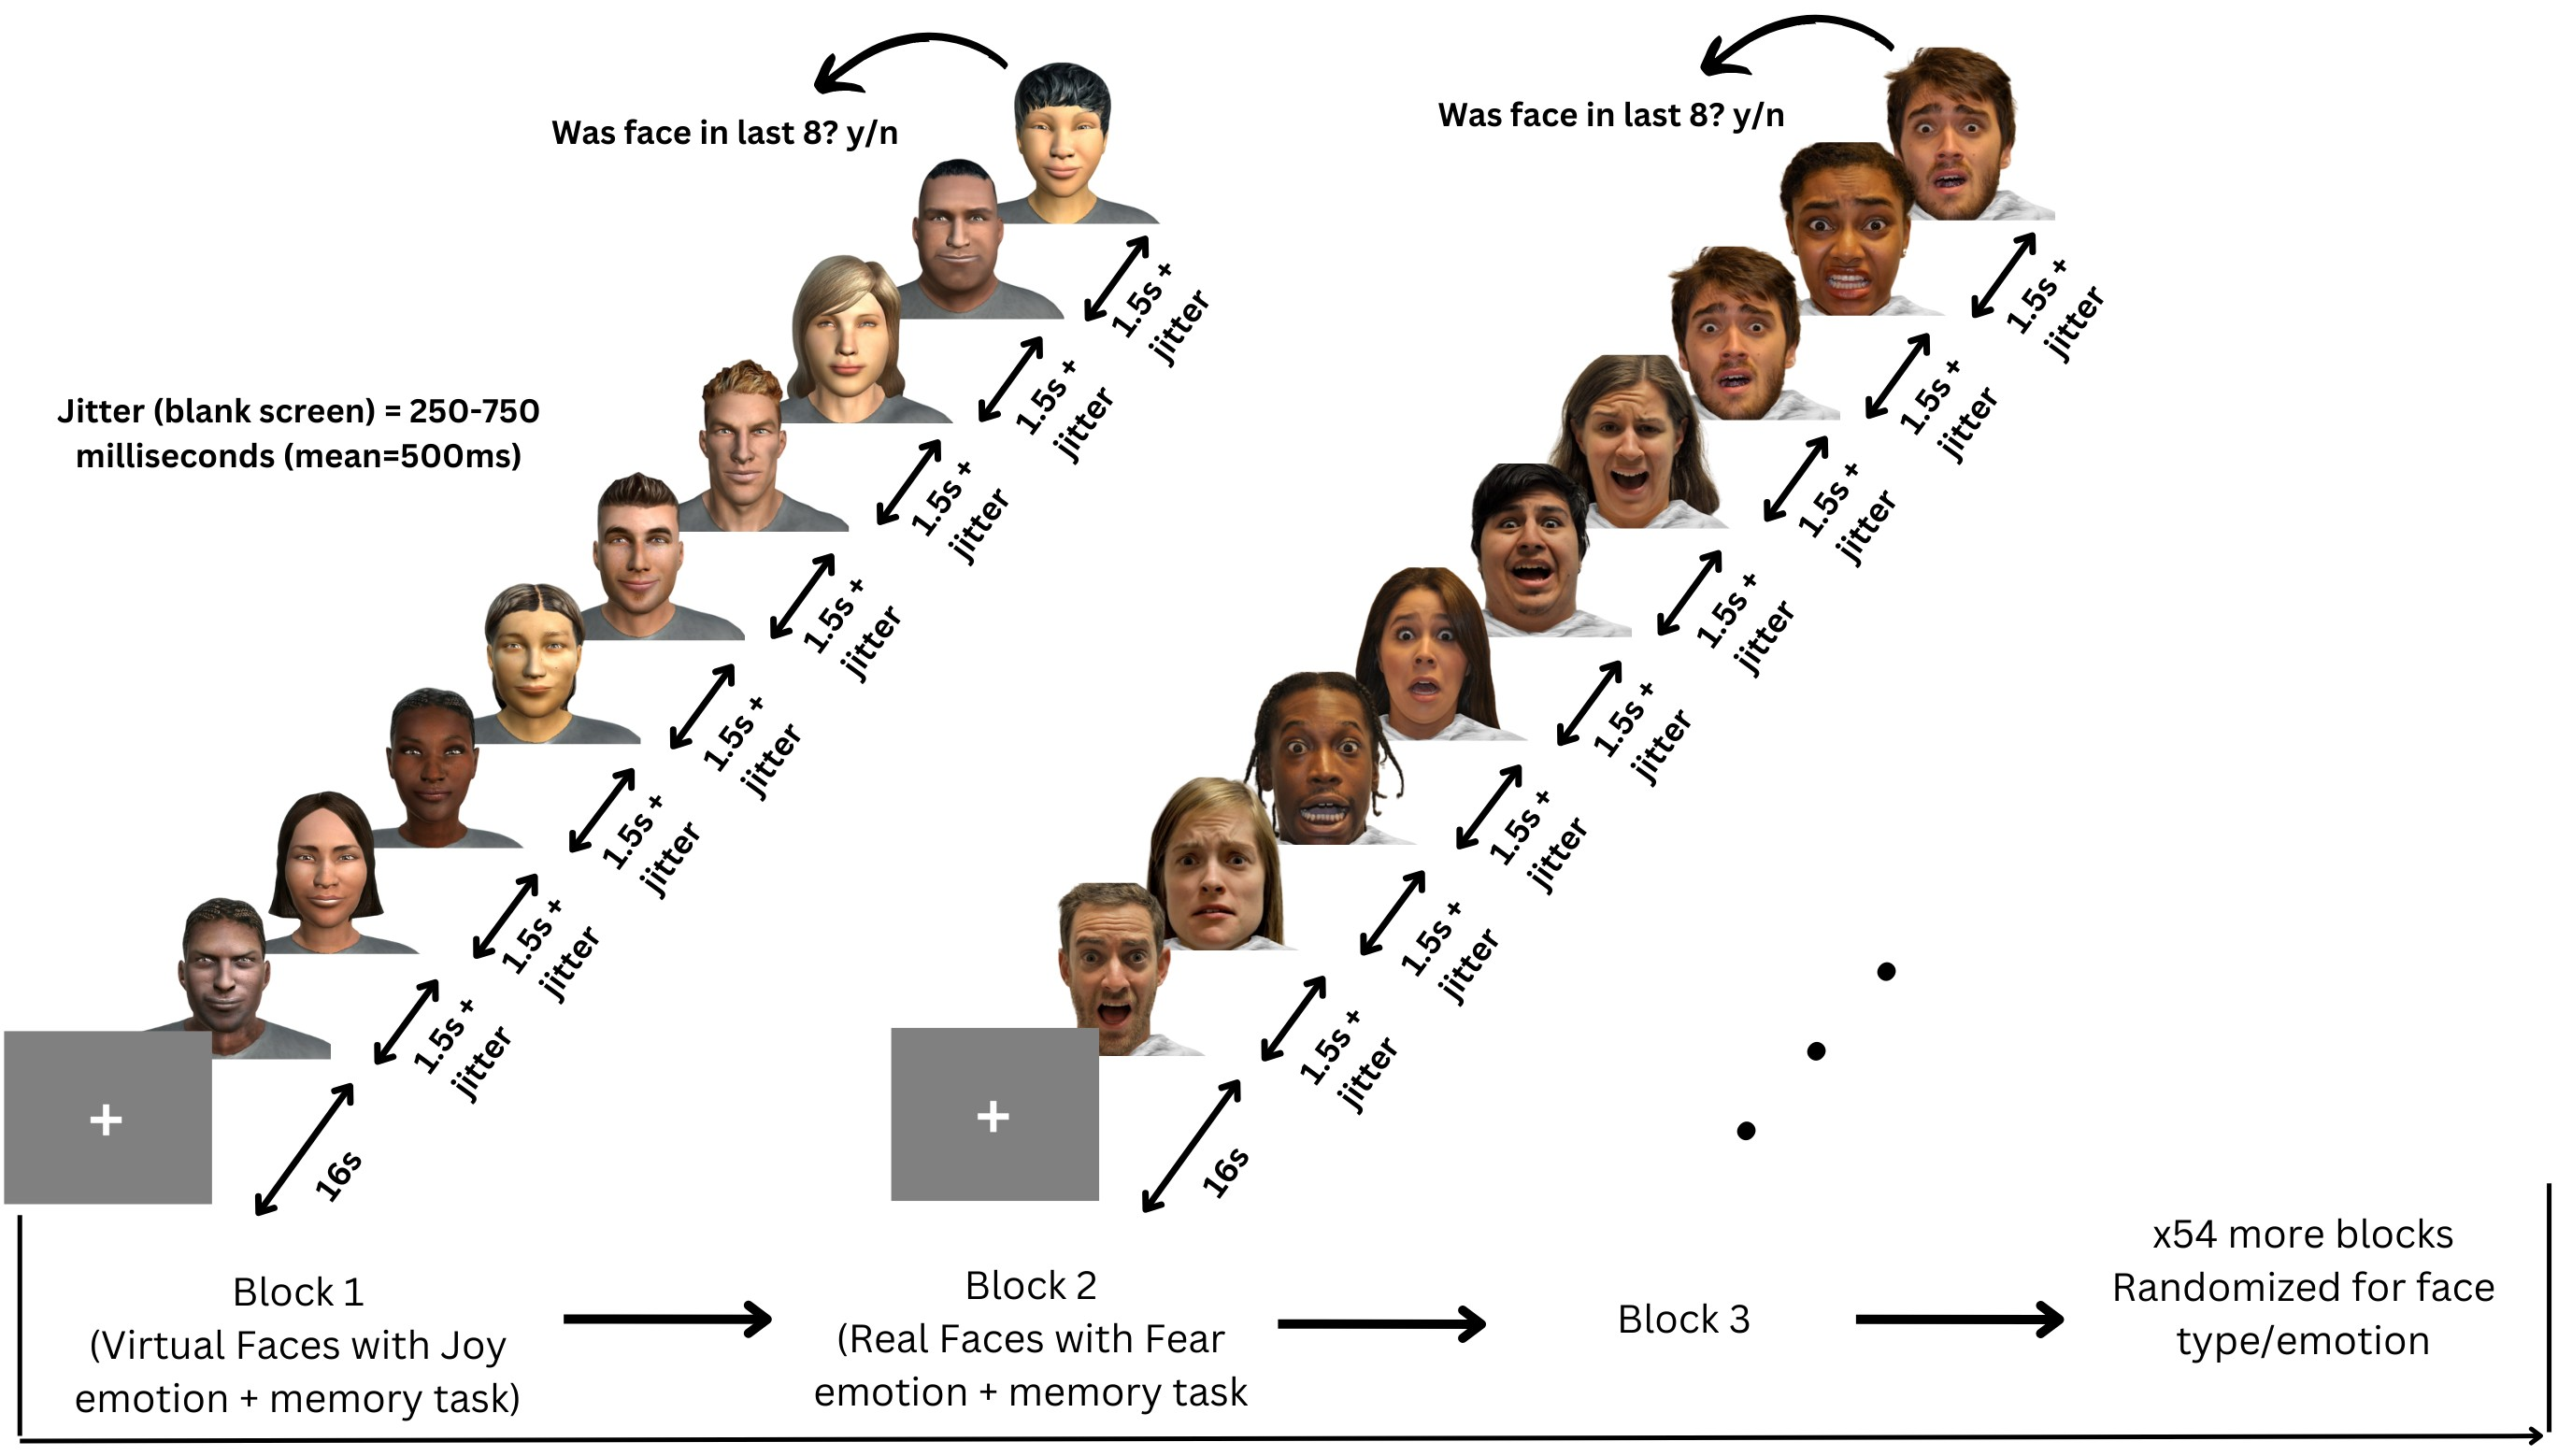
\includegraphics[width=1\textwidth]{C:/Users/super/OneDrive - Ontario Tech University/fNIRS_Emotions/plots/figures/Paradigm.jpg}
    \caption[Experimental paradigm overview]{Participants viewed 56 blocks of 8 faces, each block being either all real or all virtual faces.
    Every face in a block displayed the same emotional expression, one of: anger, disgust, fear, happiness, sadness, surprise, neutral. }
    \label{fig:paradigm}
\end{figure}

\section{Analyses}
All fNIRS data was preprocessed and analyzed with Python 3.11.9 using MNE (version 1.9.0) \citep{gramfort_meg_2013} and MNE-NIRS (version 0.7.1) \citep{luke_analysis_2021}, which used the Nilearn package (version 0.9.2). 
Data were analyzed with a General Linear Model (GLM), followed by a functional connectivity analysis.
The memory task was analyzed in Python using the statsmodels package (version 0.14.4) \citep{seabold2010statsmodels}. 
The data generated during this study has been made publicly available on the Open Science Framework: (\href{https://osf.io/d7bzp/?view_only=f5a96f051edb4e768c5e4461699ef1ce}{https://osf.io/d7bzp/?view\_only=f5a96f051edb4e768c5e4461699ef1ce}). 

\subsection{fNIRS preprocessing}
\label{sec:preprocessing}
\begin{figure}[H]
    \centering
    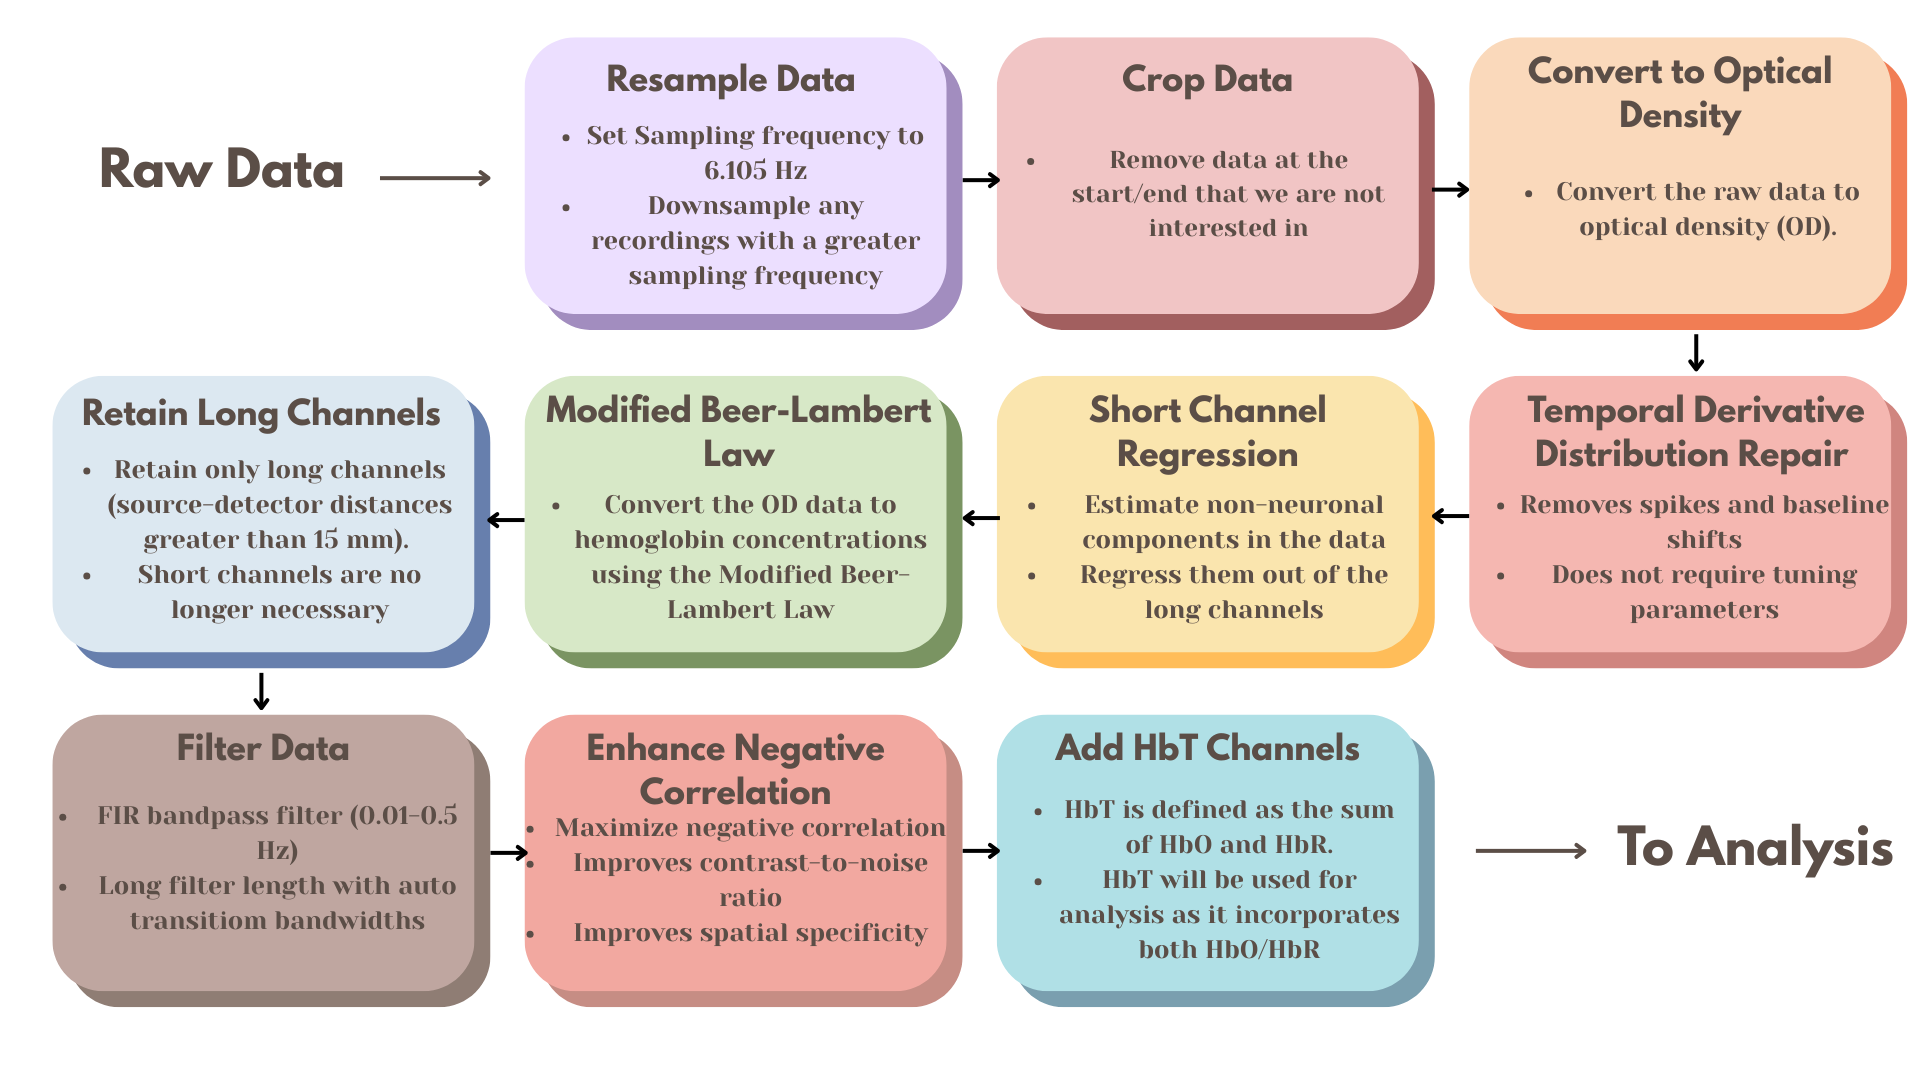
\includegraphics[width=1\textwidth]{C:/Users/super/OneDrive - Ontario Tech University/fNIRS_Emotions/plots/figures/Preprocessing Steps.png}
    \caption[Preprocessing steps for fNIRS data]{Preprocessing steps for fNIRS data, from the raw data to the fully processed data. }
    \label{fig:preprocessing_steps}
\end{figure}

The preprocessing steps for the fNIRS data, as shown in Figure \ref{fig:preprocessing_steps}, were as follows:
1) Downsample the data if the sampling frequency is greater than 6.105 Hz, the initial two datasets were sampled higher than 6.105 Hz, and the sampling frequency should be consistent across all datasets.
2) Crop the data to the first and last annotation. This gets rid of the extra data at the beginning and end of the recording that are not of interest.
3) Convert the raw data to optical density.
4) Apply temporal derivative distribution repair to the OD data \citep{fishburn_temporal_2019}. TDDR is effective at removing spikes and baseline shifts from the data. 
5) Apply short channel regression to the OD data \citep{scholkmann_measuring_2014}. Short channels are used to estimate the superficial hemodynamics (non-evoked/extracerebral/systemic components) in the data, and then regress it out of the long channels \citep{tachtsidis_false_2016}. 
6) Convert the OD data to hemoglobin concentrations using the modified Beer-Lambert law. The MBLL relates the change in light attenuation to the change in hemoglobin concentration of chromophores in the tissue \citep{kocsis_modified_2006}.
7) Retain only long channels (source-detector distance $>$ 15 mm). Since the short channels have already been regressed out, it is no longer necessary to keep them in the data.
8) This FIR bandpass filter extracts signal components in the 0.01-0.5 Hz range, it uses a long filter length (2015 samples) with automatically determined transition bandwidths by MNE-Python \citep{pinti_current_2019}. 
9) Maximizes negative correlation between HbO and HbR \citep{cui_functional_2010}. This method removes spikes, improves contrast-to-noise ratio, and improves spatial specificity of the data.
10) Add HbT (total hemoglobin) channels to the data. HbT is defined as the sum of HbO and HbR. Often, fNIRS studies will only use either one of HbO or HbR channels (more frequently HbO), leaving out one channel with no justification \citep{kinder_systematic_2022}. Therefore, HbT channels are chosen, as HbT makes use of both HbO and HbR channels, and using both hemoglobin species improves the inferences as to where activation occurs \citep{hocke_automated_2018}.

Variable length epochs were created for each block of 8 faces, which were 14-18 seconds long (mean = 16s), depending on the ISI's (see \ref{sec:Procedure}).
Epochs were sorted by Face Type (Real, Virtual), and Emotion (Anger, Disgust, Fear, Happiness, Sadness, Surprise, Neutral), and their interaction.
Baseline correction was applied to remove any constant or slowly varying offsets in the data. 
The data was annotated with the onsets and offsets of each block, along with the duration and condition of each block. 
Block data were then analysed using a GLM and Functional Connectivity analysis. 

\subsection{Activation magnitude with General Linear Model (GLM)}
\label{sec:GLM}
The General Linear Model (GLM) posits that the observed haemodynamic signal at each channel or Region of Interest (ROI) is a linear combination of task-related regressors convolved with a Hemodynamic Response Function (HRF), plus nuisance regressors (e.g., drift) and residual noise. Mathematically, 

\begin{equation}
Y = X\beta + \epsilon,
\end{equation}

where \( Y \) is the observed time series, \( X \) is the design matrix, \( \beta \) represents the parameters to estimate, and \( \epsilon \) denotes the residuals assumed to be Gaussian noise.
Estimation is performed via ordinary least squares (OLS), yielding parameter estimates that quantify condition-specific activation amplitudes.

\subsubsection{Design Matrix}
For each of the epochs, events are defined by their trial type (e.g., emotion or face type), and onsets/offsets relative to the procedure start, and duration.
The design matrix is constructed using Nilearn's \texttt{make\_first\_level\_design\_matrix} by convolving a boxcar function (based on the event timing) with a canonical HRF, which is a model of the expected haemodynamic response to neural activity.
The canonical HRF Statistical Parametric Mapping (SPM) \citep{friston_statistical_2007} is chosen to model neurovascular coupling, this model captures the stereotypical rise and fall of the BOLD/fNIRS response. 
The cosine drift model was utilized, which incorporates discrete cosine transform (DCT) basis functions into the design matrix to model and remove low-frequency drifts.
The selection of the high pass cutoff frequency is guided by the structure of the experimental design. 
The cutoff period is set to twice the duration of the longest inter-trial interval, and each fixation period between epochs (or blocks) is 16 seconds. 
Therefore, a cutoff period of 32 seconds (i.e., \texttt{high\_pass=0.03125} Hz) would be appropriate. 
This ensures that the drift model does not remove task-related signal components that occur at frequencies higher than the cutoff \citep{luke_analysis_2021}.
The design matrix \( X \) and preprocessed time series are fed into MNE's \texttt{run\_glm} function, which computes OLS estimates of \( \beta \) for each channel.

\begin{figure}[H]
    \centering
    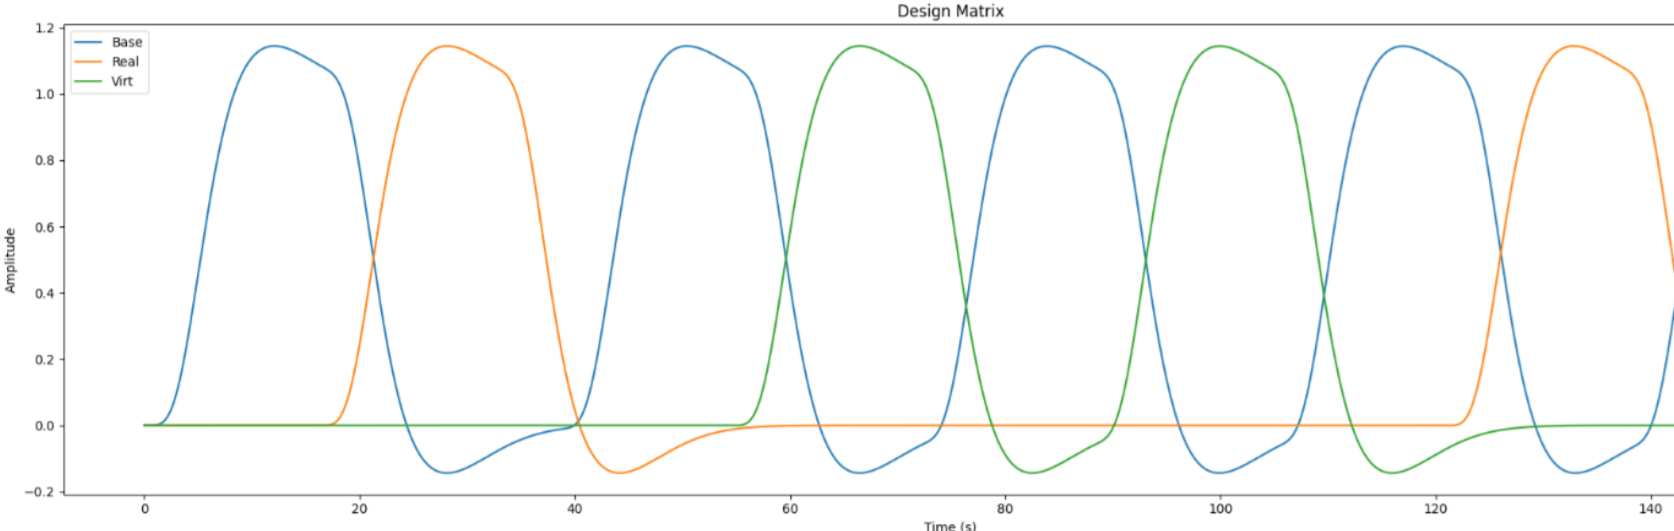
\includegraphics[width=1\textwidth]{C:/Users/super/OneDrive - Ontario Tech University/fNIRS_Emotions/plots/figures/Sample Design Matrix.png}
    \caption[Sample design matrix for GLM]{Sample design matrix for a single participant for the effect Face type, showing the first 7 blocks (250 seconds) of a single experiment.
    The design matrix is organized by condition (Blue for real, orange for virtual), this is the result of convolving the boxcar function with the canonical HRF SPM. }
    \label{fig:design_matrix}
\end{figure}

A two-way repeated measures GLM was conducted on participant's HbT responses by Face-type (2 levels: Real, Virtual) and Emotion (7 levels: Anger, Disgust, Fear, Joy, Sadness, Surprise, Neutral). 
Pairwise contrasts were then computed between conditions to identify effects of interest.

\subsubsection{Contrast Computation}
\label{sec:contrast_computation}
All pairwise contrasts were generated between conditions by constructing an identity contrast matrix over design columns. 
For each pair of conditions \( (A, B) \), the contrast vector is defined as: $c = e_A - e_B$, where \( e_A \) and \( e_B \) are the respective design matrix columns for conditions \( A \) and \( B \). 
Contrasts are computed using MNE's \texttt{compute\_contrast} function, which produces effect estimates and test statistics aggregated across channels.
Since numerous statistical tests are performed across channels and contrasts, $p$-values were FDR-corrected corrected using the Benjamini-Hochberg procedure \citep{singh_exploring_2006} with a family-wise error rate of $\alpha$=0.05.

\subsection{Network mapping with Functional Connectivity Analysis}
\label{sec:fc}
To characterize the temporal coordination between fNIRS channels during face and emotion processing, functional connectivity matrices were computed using a continuous wavelet transform (CWT)-based spectral connectivity approach.
CWT decomposes signals into simultaneous time-frequency representations, providing an optimal framework for fNIRS connectivity analysis by accommodating the non-stationary, physiological nature of hemodynamic signals. 
The morlet wavelet, a gaussian function modulated by a sine wave, was picked as they are suited to capture both slow neural rhythms and faster systemic fluctuations in fNIRS data \citep{reddy_evaluation_2021}. 
Wavelet-based approaches have been widely adopted in the fNIRS literature for connectivity and even artifact correction \citep{bergmann_evaluation_2023, hakim_quantification_2023}
Coherence combines both phase and amplitude information into a single, normalized index, 0 (no coupling) to 1 (perfect coupling), and is a richer description of coupling than phase-only or amplitude-only metrics \citep{bastos_tutorial_2016}.

For each participant, MNE's \texttt{spectral\_connectivity\_time} function was applied to compute time-resolved coherence across pairs of channels, the average of this was taken across epochs to obtain a single channel-by-channel connectivity matrix for each condition.
Each participants' connectivity matrix was then averaged across participants to obtain a group-level connectivity matrix for each condition. 
fNIRS hemodynamics predominantly fluctuate in very low frequencies (0.01-0.5 Hz) \citep{reddy_evaluation_2021}. 
The frequency range was narrowed to five evenly spaced frequences between 0.2-0.5 Hz due to short epoch length, this range still targets systemic and neurogenic oscillations while avoiding high-frequency noise \citep{xu_functional_2017}.
Averaging across these closely spaced frequencies reduces data dimensionality, simplifying downstream statistical analyses without sacrificing sensitivity to coupling dynamics. 

\subsubsection{Paired Sample t-tests}
For each mode (Face type/Emotion), and pair of conditions (e.g., Joy vs. Fear), individual-level connectivity matrices were extracted by averaging across epochs to obtain symmetric channel-by-channel coherence matrices. 
Because coherence values are bounded between 0 and 1 and exhibit skewed distributions \citep{miranda_de_sa_coherence_2009}, Fisher's r-to-z transform (\texttt{atanh}) was applied to each matrix element to normalize the data prior to parametric testing. 
Paired $t$-tests for each unique channel pair ($i > j$) were then conducted across participants using SciPy's \texttt{ttest\_rel}.
This directly tests whether mean connectivity differs between conditions, leveraging the paired design to increase statistical sensitivity \citep{hu_characterizing_2023}. 
Given the large number of channel-pair tests, and similar to the GLM analysis above in \ref{sec:contrast_computation}, $p$-values were FDR-corrected using the Benjamini-Hochberg procedure \citep{singh_exploring_2006} with a family-wise error rate of $\alpha$=0.05.

\subsubsection{ROI Chord Plots}
To distill high-dimensional channel-by-channel connectivity into interpretable inter-regional summaries, we mapped individual fNIRS channels onto anatomically defined ROI's. 
This includes left and right frontal, central/temporal, parietal, occipital regions of the brain as shown in Figure \ref{fig:brain_region_map}, and the channels were grouped into these regions based on their location in the montage.
Since multiple channels may map to the same pair of regions (e.g., several left central/temporal channels connecting to several right occipital channels), we calculated the sum of all signicant channel-pair connections for each ROI pair (separately for positive and negative $t$-values). 
We then subtracted the negative sum from the positive sum, resulting in a single integer representing the net connectivity which was positive if the positive connections outweigh the negative ones, and vice versa.
We then took the top 15\% percentile of each net connectivity value, and set the rest to zero, to show only the strongest connections between regions.
The lines were then plotted using a chord diagram, with the line color indicating the direction of the net connectivity (positive or negative), and the line width indicating the magnitude of the net connectivity (the absolute value of the net connectivity).

\subsubsection{Emotion Summary Ratio Plot}
To summarize the net connectivity between regions for each emotion, we calculated a ratio of positive to negative connections for each emotion pair.
The ratio was calculated by taking the difference of the count of significant channels where the $t$-value was positive and the count of significant channels where the $t$-value was negative, and dividing it by the total number of significant channels for that emotion pair. 
This ratio provides a measure of the net connectivity across all ROI's for each emotion, with a positive ratio indicating that one emotion has a stronger net connectivity than the other, and a negative ratio indicating that the other emotion has a stronger net connectivity.

\subsubsection{Region Summary Plot}
To summarize the net connectivity across all emotions for each region, we summed the number of significantly different channel pairs between each region pair across all emotions, disregarding the direction of the $t$-value.
This provides a measure of the net connectivity across all emotions for each region, showing which regions are more connected across all emotions.
The 3 regions with the highest and lowest number of significant channel pairs are marked, to emphasize the most/least connected regions across all emotions.

\subsection{Memory Task Analysis}
\label{sec:memory_task_analysis}
Raw behavioral data captured from PsychoPy were preprocessed to identify participant keyboard responses. 
The total correct trials per participant were summed. 
Since each block of faces was either all real or all virtual, and all had the same emotional expression (as discussed in \ref{sec:Procedure}), each y/n response was labeled with Face type and Emotion.
An OLS model was fit with accuracy (converted to numeric 0/1) as the dependent variable and categorical predictors for Face Type, Emotion, and their interaction. 
The goal is to determine the main effects of these two factors individually, as well as their interaction, on response accuracy.
A two-way Type III ANOVA (via \texttt{sm.stats.anova\_lm(model, typ=3)}) provided $F$-statistics and $p$-values for main effects and interaction.
This version of the ANOVA is especially suitable when interactions are included in the model, as it calculates each effect after accounting for all other terms.